\documentclass{article}
% this document previews all of the tikzit figures I have made in one pdf, the names are printed before the figures



% this is the preamble created by tikzit, we can edit this in the final document to change the shapes we use for nodes, edge styles, etc... 
% just be sure to use the same name for the same kind of node/edge in any figures you make


\usepackage[svgnames]{xcolor}
\usepackage{tikz}
\usetikzlibrary{decorations.markings}
\usetikzlibrary{shapes.geometric}
%\pagestyle{empty}

\newcommand\scaledLW{0.5} % scaled linewidth for fig 2, defined globally so they can be changed easily

\newcommand\scaledNodeSize{0.5} % scaled node size for fig 2, defined globally so they can be changed easily

\pgfdeclarelayer{edgelayer}
\pgfdeclarelayer{nodelayer}
\pgfsetlayers{edgelayer,nodelayer,main}

\tikzstyle{none}=[inner sep=0pt]

\tikzstyle{rn}=[circle,fill=Red,draw=Black,line width=0.8 pt]
\tikzstyle{gn}=[circle,fill=Lime,draw=Black,line width=0.8 pt]
\tikzstyle{yn}=[circle,fill=Yellow,draw=Black,line width=0.8 pt]
\tikzstyle{auxiliary_qubit}=[circle,fill=Red,draw=Black,scale=0.8]
\tikzstyle{logical_qubit}=[circle,fill=Black,draw=Black,scale=0.8]
\tikzstyle{emb_logical_qubit}=[circle,fill=Black,draw=Black,scale=0.8,line width=2.000]
\tikzstyle{emb_auxiliary_qubit}=[circle,fill=Red,draw=Black,scale=0.8,line width=2.000]
\tikzstyle{unused_qubit}=[circle,fill=Gray,draw=Gray,scale=0.8]
\tikzstyle{arrow_end}=[circle,fill=none,draw=none,scale=.1]




\tikzstyle{simple}=[-,draw=Black,line width=1.000]
\tikzstyle{added}=[-,draw=Black,line width=1.000]
%\tikzstyle{added}=[-,draw=green,line width=1.000]
\definecolor{tempcolor}{rgb}{.9,.9,.9}
\tikzstyle{unused}=[-,draw=tempcolor,line width=0.500]
%\definecolor{tempcolor}{rgb}{.7,.9,.7}
%\tikzstyle{unused_added}=[-,draw=tempcolor,line width=1.000]
%\tikzstyle{unused_added}=[-,draw=green,draw opacity=1,line width=1.000,dashed]
%\tikzstyle{unused_added}=[-,draw=cyan,draw opacity=1,line width=0.5]
\tikzstyle{unused_added}=[-,draw=tempcolor,draw opacity=1,line width=0.5]
\tikzstyle{embedding}=[-,draw=Black,line width=3.250]
\tikzstyle{arrow}=[-,draw=Black,postaction={decorate},decoration={markings,mark=at position .5 with {\arrow{>}}},line width=2.000]


 % input the globally used tikz preamble

\usepackage{float}
\floatplacement{figure}{H} % forces all floats to be positioned where the command which calls them is used

\begin{document}

\begin{figure}
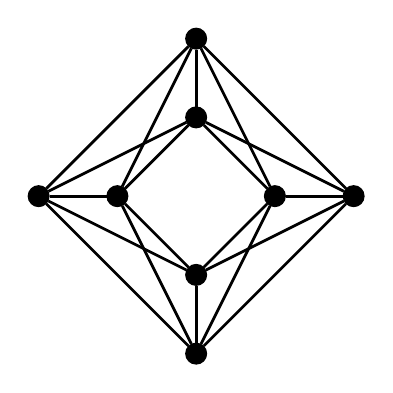
\begin{tikzpicture}
	\begin{pgfonlayer}{nodelayer}
		\node [style=logical_qubit] (0) at (0, 2) {};
		\node [style=logical_qubit] (1) at (0, 1) {};
		\node [style=logical_qubit] (2) at (-2, -0) {};
		\node [style=logical_qubit] (3) at (-1, -0) {};
		\node [style=logical_qubit] (4) at (1, -0) {};
		\node [style=logical_qubit] (5) at (2, -0) {};
		\node [style=logical_qubit] (6) at (0, -1) {};
		\node [style=logical_qubit] (7) at (0, -2) {};
	\end{pgfonlayer}
	\begin{pgfonlayer}{edgelayer}
		\draw [style=simple] (7) to (5);
		\draw [style=simple] (5) to (0);
		\draw [style=simple] (0) to (2);
		\draw [style=simple] (7) to (2);
		\draw [style=simple] (7) to (3);
		\draw [style=simple] (7) to (4);
		\draw [style=simple] (6) to (3);
		\draw [style=simple] (6) to (2);
		\draw [style=simple] (6) to (4);
		\draw [style=simple] (4) to (1);
		\draw [style=simple] (3) to (1);
		\draw [style=simple] (6) to (5);
		\draw [style=simple] (4) to (0);
		\draw [style=simple] (3) to (0);
		\draw [style=simple] (1) to (2);
		\draw [style=simple] (1) to (5);
		\draw [style=added] (2) to (3);
		\draw [style=added] (0) to (1);
		\draw [style=added] (4) to (5);
		\draw [style=added] (6) to (7);
	\end{pgfonlayer}
\end{tikzpicture}

\caption{pegasus\_v\_chimera\_uc.tikz: shows extra edges added to chimera unit cell to make Pegasus unit cell}
\end{figure}

\begin{figure}
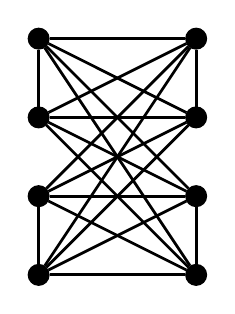
\begin{tikzpicture}
	\begin{pgfonlayer}{nodelayer}
		\node [style=logical_qubit] (0) at (0, 3) {};
		\node [style=logical_qubit] (1) at (0, 2) {};
		\node [style=logical_qubit] (2) at (2, 3) {};
		\node [style=logical_qubit] (3) at (2, 2) {};
		\node [style=logical_qubit] (4) at (2, 1) {};
		\node [style=logical_qubit] (5) at (2, -0) {};
		\node [style=logical_qubit] (6) at (0, 1) {};
		\node [style=logical_qubit] (7) at (0, -0) {};
	\end{pgfonlayer}
	\begin{pgfonlayer}{edgelayer}
		\draw [style=simple] (7) to (5);
		\draw [style=simple] (5) to (0);
		\draw [style=simple] (0) to (2);
		\draw [style=simple] (7) to (2);
		\draw [style=simple] (7) to (3);
		\draw [style=simple] (7) to (4);
		\draw [style=simple] (6) to (3);
		\draw [style=simple] (6) to (2);
		\draw [style=simple] (6) to (4);
		\draw [style=simple] (4) to (1);
		\draw [style=simple] (3) to (1);
		\draw [style=simple] (6) to (5);
		\draw [style=simple] (4) to (0);
		\draw [style=simple] (3) to (0);
		\draw [style=simple] (1) to (2);
		\draw [style=simple] (1) to (5);
		\draw [style=added] (2) to (3);
		\draw [style=added] (0) to (1);
		\draw [style=added] (4) to (5);
		\draw [style=added] (6) to (7);
	\end{pgfonlayer}
\end{tikzpicture}

\caption{pegasus\_v\_chimera\_uc\_k44.tikz: shows extra edges added to chimera unit cell to make Pegasus unit cell}
\end{figure}


\begin{figure}
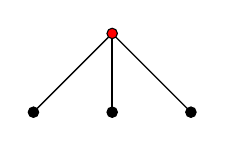
\begin{tikzpicture}[every node/.style={scale=\scaledNodeSize}]

	\begin{pgfonlayer}{nodelayer}
		\node [style=auxiliary_qubit] (0) at (0, 5) {};
		\node [style=logical_qubit] (1) at (-1, 4) {};
		\node [style=logical_qubit] (2) at (0, 4) {};
		\node [style=logical_qubit] (3) at (1, 4) {};
	\end{pgfonlayer}
	\begin{pgfonlayer}{edgelayer}
		\draw [style=simple,line width=\scaledLW] (1) to (0);
		\draw [style=simple,line width=\scaledLW] (0) to (2);
		\draw [style=simple,line width=\scaledLW] (0) to (3);
	\end{pgfonlayer}
\end{tikzpicture}

\caption{all\_to\_aux.tikz}
\end{figure}

\begin{figure}
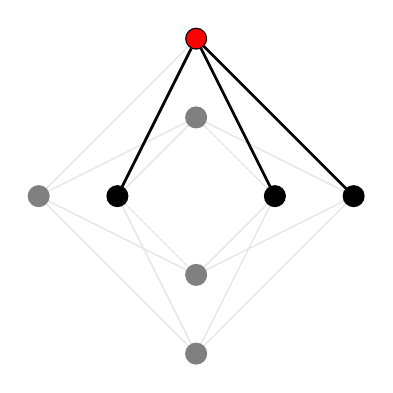
\begin{tikzpicture}
	\begin{pgfonlayer}{nodelayer}
		\node [style={auxiliary_qubit}] (0) at (0, 2) {};
		\node [style={unused_qubit}] (1) at (0, 1) {};
		\node [style={unused_qubit}] (2) at (0, -2) {};
		\node [style={logical_qubit}] (3) at (1, 0) {};
		\node [style={logical_qubit}] (4) at (-1, 0) {};
		\node [style={unused_qubit}] (5) at (-2, 0) {};
		\node [style={unused_qubit}] (6) at (0, -1) {};
		\node [style={logical_qubit}] (7) at (2, 0) {};
	\end{pgfonlayer}
	\begin{pgfonlayer}{edgelayer}
		\draw [style=unused] (1) to (3);
		\draw [style=unused] (0) to (5);
		\draw [style=unused] (5) to (2);
		\draw [style=unused] (5) to (1);
		\draw [style=unused] (6) to (3);
		\draw [style=unused] (6) to (4);
		\draw [style=unused] (6) to (5);
		\draw [style=unused] (6) to (7);
		\draw [style=unused] (7) to (2);
		\draw [style=unused] (1) to (7);
		\draw [style=unused] (3) to (2);
		\draw [style=unused] (1) to (4);
		\draw [style=unused] (4) to (2);
		\draw [style=simple] (0) to (7);
		\draw [style=simple] (0) to (3);
		\draw [style=simple] (4) to (0);
	\end{pgfonlayer}
\end{tikzpicture}

\caption{all\_to\_aux\_chimera.tikz}
\end{figure}

Gadgets with adjacency graph corresponding to all\_to\_aux.tikz(\scalebox{.25}{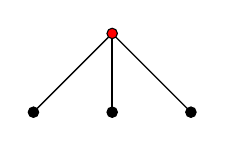
\begin{tikzpicture}[every node/.style={scale=\scaledNodeSize}]

	\begin{pgfonlayer}{nodelayer}
		\node [style=auxiliary_qubit] (0) at (0, 5) {};
		\node [style=logical_qubit] (1) at (-1, 4) {};
		\node [style=logical_qubit] (2) at (0, 4) {};
		\node [style=logical_qubit] (3) at (1, 4) {};
	\end{pgfonlayer}
	\begin{pgfonlayer}{edgelayer}
		\draw [style=simple,line width=\scaledLW] (1) to (0);
		\draw [style=simple,line width=\scaledLW] (0) to (2);
		\draw [style=simple,line width=\scaledLW] (0) to (3);
	\end{pgfonlayer}
\end{tikzpicture}
}):

\begin{itemize}
\item NTR-KZFD
\item NTR-ABCG
\end{itemize}

\begin{figure}
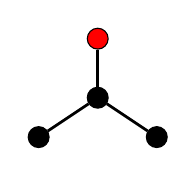
\begin{tikzpicture}
	\begin{pgfonlayer}{nodelayer}
		\node [style=logical_qubit] (0) at (0, -0) {};
		\node [style=auxiliary_qubit] (1) at (0, 0.75) {};
		\node [style=logical_qubit] (2) at (0.75, -0.5) {};
		\node [style=logical_qubit] (3) at (-0.75, -0.5) {};
	\end{pgfonlayer}
	\begin{pgfonlayer}{edgelayer}
		\draw [style=simple] (2) to (0);
		\draw [style=simple] (3) to (0);
		\draw [style=simple] (1) to (0);
	\end{pgfonlayer}
\end{tikzpicture}

\caption{logical\_fork.tikz}
\end{figure}

\begin{figure}
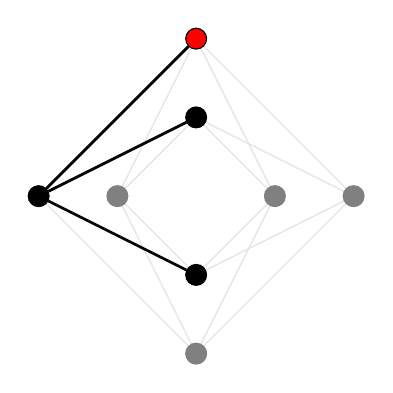
\begin{tikzpicture}
	\begin{pgfonlayer}{nodelayer}
		\node [style=logical_qubit] (0) at (-2, -0) {};
		\node [style=unused_qubit] (1) at (-1, -0) {};
		\node [style=unused_qubit] (2) at (2, -0) {};
		\node [style=logical_qubit] (3) at (0, 1) {};
		\node [style=logical_qubit] (4) at (0, -1) {};
		\node [style=unused_qubit] (5) at (0, -2) {};
		\node [style=unused_qubit] (6) at (1, -0) {};
		\node [style=auxiliary_qubit] (7) at (0, 2) {};
	\end{pgfonlayer}
	\begin{pgfonlayer}{edgelayer}
		\draw [style=unused] (0) to (5);
		\draw [style=unused] (5) to (2);
		\draw [style=unused] (5) to (1);
		\draw [style=unused] (6) to (3);
		\draw [style=unused] (6) to (4);
		\draw [style=unused] (6) to (5);
		\draw [style=unused] (1) to (3);
		\draw [style=unused] (3) to (2);
		\draw [style=unused] (1) to (4);
		\draw [style=unused] (4) to (2);
		\draw [style=unused] (6) to (7);
		\draw [style=unused] (7) to (2);
		\draw [style=unused] (1) to (7);
		\draw [style=simple] (0) to (3);
		\draw [style=simple] (4) to (0);
		\draw [style=simple] (0) to (7);	
	\end{pgfonlayer}
\end{tikzpicture}

\caption{logical\_fork\_chimera.tikz}
\end{figure}

Gadgets with adjacency graph corresponding to logical\_fork.tikz(\scalebox{.25}{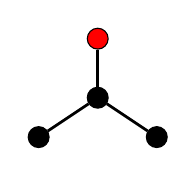
\begin{tikzpicture}
	\begin{pgfonlayer}{nodelayer}
		\node [style=logical_qubit] (0) at (0, -0) {};
		\node [style=auxiliary_qubit] (1) at (0, 0.75) {};
		\node [style=logical_qubit] (2) at (0.75, -0.5) {};
		\node [style=logical_qubit] (3) at (-0.75, -0.5) {};
	\end{pgfonlayer}
	\begin{pgfonlayer}{edgelayer}
		\draw [style=simple] (2) to (0);
		\draw [style=simple] (3) to (0);
		\draw [style=simple] (1) to (0);
	\end{pgfonlayer}
\end{tikzpicture}
}):

\begin{itemize}
\item NTR-ABCB
\end{itemize}

\begin{figure}
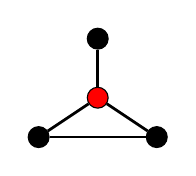
\begin{tikzpicture}
	\begin{pgfonlayer}{nodelayer}
		\node [style=auxiliary_qubit] (0) at (0, -0) {};
		\node [style=logical_qubit] (1) at (0, 0.75) {};
		\node [style=logical_qubit] (2) at (0.75, -0.5) {};
		\node [style=logical_qubit] (3) at (-0.75, -0.5) {};
	\end{pgfonlayer}
	\begin{pgfonlayer}{edgelayer}
		\draw [style=simple] (2) to (0);
		\draw [style=simple] (3) to (0);
		\draw [style=simple] (1) to (0);
		\draw [style=simple] (3) to (2);
	\end{pgfonlayer}
\end{tikzpicture}

\caption{k4\_missing\_2edge.tikz}
\end{figure}

\begin{figure}
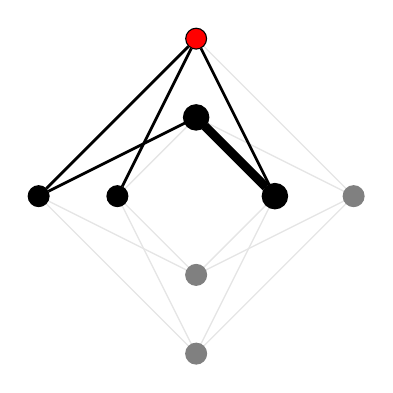
\begin{tikzpicture}
	\begin{pgfonlayer}{nodelayer}
		\node [style={logical_qubit}] (0) at (-2, -0) {};
		\node [style={logical_qubit}] (1) at (-1, -0) {};
		\node [style=unused_qubit] (2) at (2, -0) {};
		\node [style={emb_logical_qubit}] (3) at (0, 1) {};
		\node [style=unused_qubit] (4) at (0, -1) {};
		\node [style=unused_qubit] (5) at (0, -2) {};
		\node [style={emb_logical_qubit}] (6) at (1, -0) {};
		\node [style={auxiliary_qubit}] (7) at (0, 2) {};
	\end{pgfonlayer}
	\begin{pgfonlayer}{edgelayer}
		\draw [style=unused] (1) to (3);
		\draw [style=simple] (0) to (3);
		\draw [style=unused] (3) to (2);
		\draw [style=unused] (1) to (4);
		\draw [style=unused] (4) to (2);
		\draw [style=unused] (4) to (0);
		\draw [style=unused] (0) to (5);
		\draw [style=unused] (5) to (2);
		\draw [style=unused] (5) to (1);
		\draw [style={embedding}] (6) to (3);
		\draw [style=unused] (6) to (4);
		\draw [style=unused] (6) to (5);
		\draw [style=simple] (0) to (7);
		\draw [style=simple] (6) to (7);
		\draw [style=unused] (7) to (2);
		\draw [style=simple] (1) to (7);
	\end{pgfonlayer}
\end{tikzpicture}

\caption{k4\_missing\_2edge\_chimera.tikz}
\end{figure}

Gadgets with adjacency graph corresponding to k4\_missing\_2edge.tikz(\scalebox{.25}{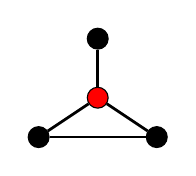
\begin{tikzpicture}
	\begin{pgfonlayer}{nodelayer}
		\node [style=auxiliary_qubit] (0) at (0, -0) {};
		\node [style=logical_qubit] (1) at (0, 0.75) {};
		\node [style=logical_qubit] (2) at (0.75, -0.5) {};
		\node [style=logical_qubit] (3) at (-0.75, -0.5) {};
	\end{pgfonlayer}
	\begin{pgfonlayer}{edgelayer}
		\draw [style=simple] (2) to (0);
		\draw [style=simple] (3) to (0);
		\draw [style=simple] (1) to (0);
		\draw [style=simple] (3) to (2);
	\end{pgfonlayer}
\end{tikzpicture}
}):

\begin{itemize}
\item Asymmetric reduction
\end{itemize}

\begin{figure}
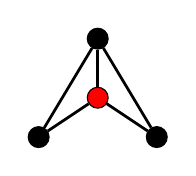
\begin{tikzpicture}
	\begin{pgfonlayer}{nodelayer}
		\node [style=auxiliary_qubit] (0) at (0, -0) {};
		\node [style=logical_qubit] (1) at (0, 0.75) {};
		\node [style=logical_qubit] (2) at (0.75, -0.5) {};
		\node [style=logical_qubit] (3) at (-0.75, -0.5) {};
	\end{pgfonlayer}
	\begin{pgfonlayer}{edgelayer}
		\draw [style=simple] (3) to (1);
		\draw [style=simple] (1) to (2);
		\draw [style=simple] (2) to (0);
		\draw [style=simple] (3) to (0);
		\draw [style=simple] (1) to (0);
	\end{pgfonlayer}
\end{tikzpicture}

\caption{k4\_missing\_edge.tikz}
\end{figure}

\begin{figure}
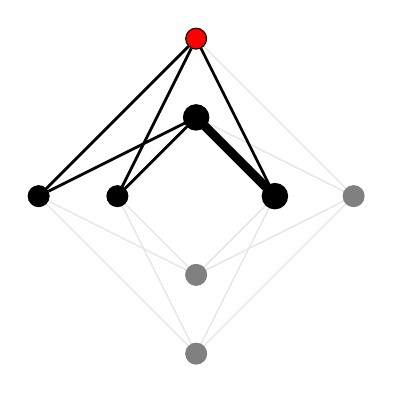
\begin{tikzpicture}
	\begin{pgfonlayer}{nodelayer}
		\node [style={logical_qubit}] (0) at (-2, -0) {};
		\node [style={logical_qubit}] (1) at (-1, -0) {};
		\node [style=unused_qubit] (2) at (2, -0) {};
		\node [style={emb_logical_qubit}] (3) at (0, 1) {};
		\node [style=unused_qubit] (4) at (0, -1) {};
		\node [style=unused_qubit] (5) at (0, -2) {};
		\node [style={emb_logical_qubit}] (6) at (1, -0) {};
		\node [style={auxiliary_qubit}] (7) at (0, 2) {};
	\end{pgfonlayer}
	\begin{pgfonlayer}{edgelayer}
		\draw [style=simple] (1) to (3);
		\draw [style=simple] (0) to (3);
		\draw [style=unused] (3) to (2);
		\draw [style=unused] (1) to (4);
		\draw [style=unused] (4) to (2);
		\draw [style=unused] (4) to (0);
		\draw [style=unused] (0) to (5);
		\draw [style=unused] (5) to (2);
		\draw [style=unused] (5) to (1);
		\draw [style={embedding}] (6) to (3);
		\draw [style=unused] (6) to (4);
		\draw [style=unused] (6) to (5);
		\draw [style=simple] (0) to (7);
		\draw [style=simple] (6) to (7);
		\draw [style=unused] (7) to (2);
		\draw [style=simple] (1) to (7);
	\end{pgfonlayer}
\end{tikzpicture}

\caption{k4\_missing\_edge\_chimera.tikz}
\end{figure}

Gadgets with adjacency graph corresponding to k4\_missing\_edge.tikz(\scalebox{.25}{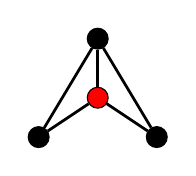
\begin{tikzpicture}
	\begin{pgfonlayer}{nodelayer}
		\node [style=auxiliary_qubit] (0) at (0, -0) {};
		\node [style=logical_qubit] (1) at (0, 0.75) {};
		\node [style=logical_qubit] (2) at (0.75, -0.5) {};
		\node [style=logical_qubit] (3) at (-0.75, -0.5) {};
	\end{pgfonlayer}
	\begin{pgfonlayer}{edgelayer}
		\draw [style=simple] (3) to (1);
		\draw [style=simple] (1) to (2);
		\draw [style=simple] (2) to (0);
		\draw [style=simple] (3) to (0);
		\draw [style=simple] (1) to (0);
	\end{pgfonlayer}
\end{tikzpicture}
}):

\begin{itemize}
\item Asymmetric cubic reduction
\end{itemize}

\begin{figure}
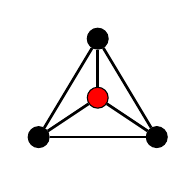
\begin{tikzpicture}
	\begin{pgfonlayer}{nodelayer}
		\node [style=auxiliary_qubit] (0) at (0, -0) {};
		\node [style=logical_qubit] (1) at (0, 0.75) {};
		\node [style=logical_qubit] (2) at (0.75, -0.5) {};
		\node [style=logical_qubit] (3) at (-0.75, -0.5) {};
	\end{pgfonlayer}
	\begin{pgfonlayer}{edgelayer}
		\draw [style=simple] (3) to (1);
		\draw [style=simple] (1) to (2);
		\draw [style=simple] (2) to (0);
		\draw [style=simple] (3) to (0);
		\draw [style=simple] (1) to (0);
		\draw [style=simple] (3) to (2);
	\end{pgfonlayer}
\end{tikzpicture}

\caption{k4.tikz}
\end{figure}

\begin{figure}
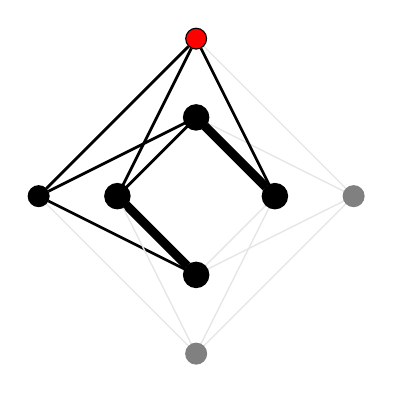
\begin{tikzpicture}
	\begin{pgfonlayer}{nodelayer}
		\node [style={logical_qubit}] (0) at (-2, -0) {};
		\node [style={emb_logical_qubit}] (1) at (-1, -0) {};
		\node [style=unused_qubit] (2) at (2, -0) {};
		\node [style={emb_logical_qubit}] (3) at (0, 1) {};
		\node [style={emb_logical_qubit}] (4) at (0, -1) {};
		\node [style=unused_qubit] (5) at (0, -2) {};
		\node [style={emb_logical_qubit}] (6) at (1, -0) {};
		\node [style={auxiliary_qubit}] (7) at (0, 2) {};
	\end{pgfonlayer}
	\begin{pgfonlayer}{edgelayer}
		\draw [style=simple] (1) to (3);
		\draw [style=simple] (0) to (3);
		\draw [style=unused] (3) to (2);
		\draw [style={embedding}] (1) to (4);
		\draw [style=unused] (4) to (2);
		\draw [style=simple] (4) to (0);
		\draw [style=unused] (0) to (5);
		\draw [style=unused] (5) to (2);
		\draw [style=unused] (5) to (1);
		\draw [style={embedding}] (6) to (3);
		\draw [style=unused] (6) to (4);
		\draw [style=unused] (6) to (5);
		\draw [style=simple] (0) to (7);
		\draw [style=simple] (6) to (7);
		\draw [style=unused] (7) to (2);
		\draw [style=simple] (1) to (7);
	\end{pgfonlayer}
\end{tikzpicture}

\caption{k4\_chimera.tikz}
\end{figure}


Gadgets with adjacency graph corresponding to k4.tikz(\scalebox{.25}{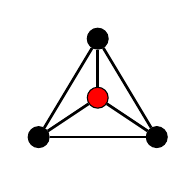
\begin{tikzpicture}
	\begin{pgfonlayer}{nodelayer}
		\node [style=auxiliary_qubit] (0) at (0, -0) {};
		\node [style=logical_qubit] (1) at (0, 0.75) {};
		\node [style=logical_qubit] (2) at (0.75, -0.5) {};
		\node [style=logical_qubit] (3) at (-0.75, -0.5) {};
	\end{pgfonlayer}
	\begin{pgfonlayer}{edgelayer}
		\draw [style=simple] (3) to (1);
		\draw [style=simple] (1) to (2);
		\draw [style=simple] (2) to (0);
		\draw [style=simple] (3) to (0);
		\draw [style=simple] (1) to (0);
		\draw [style=simple] (3) to (2);
	\end{pgfonlayer}
\end{tikzpicture}
}):

\begin{itemize}
\item PTR-Ishikawa
\item PTR-BCR (1-4)
\item PTR-KZ
\item Z version of PTR-KZ 
\end{itemize}

\begin{figure}
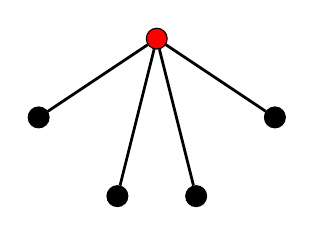
\begin{tikzpicture}
	\begin{pgfonlayer}{nodelayer}
		\node [style=logical_qubit] (0) at (-1, -0) {};
		\node [style=logical_qubit] (1) at (0, -1) {};
		\node [style=logical_qubit] (2) at (1, -1) {};
		\node [style=logical_qubit] (3) at (2, -0) {};
		\node [style=auxiliary_qubit] (4) at (0.5, 1) {};
	\end{pgfonlayer}
	\begin{pgfonlayer}{edgelayer}
		\draw [style=simple] (0) to (4);
		\draw [style=simple] (1) to (4);
		\draw [style=simple] (2) to (4);
		\draw [style=simple] (4) to (3);
	\end{pgfonlayer}
\end{tikzpicture}

\caption{all\_to\_aux4.tikz}
\end{figure}

\begin{figure}
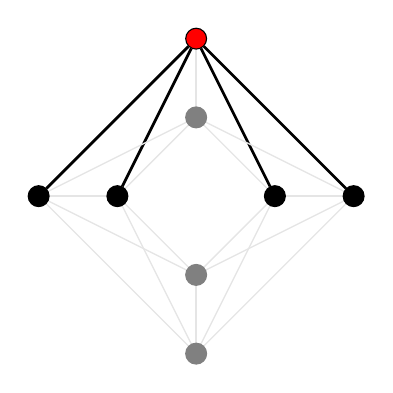
\begin{tikzpicture}
	\begin{pgfonlayer}{nodelayer}
		\node [style=logical_qubit] (0) at (-2, -0) {};
		\node [style=logical_qubit] (1) at (-1, -0) {};
		\node [style=logical_qubit] (2) at (1, -0) {};
		\node [style=logical_qubit] (3) at (2, -0) {};
		\node [style=auxiliary_qubit] (4) at (0, 2) {};
		\node [style=unused_qubit] (5) at (0, 1) {};
		\node [style=unused_qubit] (6) at (0, -1) {};
		\node [style=unused_qubit] (7) at (0, -2) {};
	\end{pgfonlayer}
	\begin{pgfonlayer}{edgelayer}
		\draw [style=simple] (0) to (4);
		\draw [style=simple] (1) to (4);
		\draw [style=simple] (2) to (4);
		\draw [style=simple] (4) to (3);
		\draw [style=unused] (1) to (5);
		\draw [style=unused] (2) to (5);
		\draw [style=unused] (0) to (5);
		\draw [style=unused] (5) to (3);
		\draw [style={unused_added}] (0) to (1);
		\draw [style={unused_added}] (2) to (3);
		\draw [style=unused] (1) to (6);
		\draw [style=unused] (6) to (2);
		\draw [style=unused] (6) to (3);
		\draw [style=unused] (6) to (0);
		\draw [style=unused] (0) to (7);
		\draw [style=unused] (7) to (3);
		\draw [style=unused] (7) to (2);
		\draw [style=unused] (7) to (1);
		\draw [style={unused_added}] (4) to (5);
		\draw [style={unused_added}] (6) to (7);
	\end{pgfonlayer}
\end{tikzpicture}

\caption{all\_to\_aux4\_inPegasus.tikz}
\end{figure}

Gadgets with adjacency graph corresponding to all\_to\_aux4.tikz(\scalebox{.25}{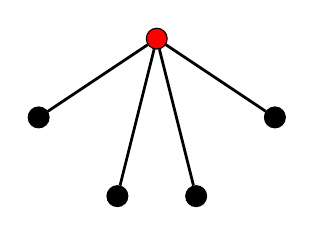
\begin{tikzpicture}
	\begin{pgfonlayer}{nodelayer}
		\node [style=logical_qubit] (0) at (-1, -0) {};
		\node [style=logical_qubit] (1) at (0, -1) {};
		\node [style=logical_qubit] (2) at (1, -1) {};
		\node [style=logical_qubit] (3) at (2, -0) {};
		\node [style=auxiliary_qubit] (4) at (0.5, 1) {};
	\end{pgfonlayer}
	\begin{pgfonlayer}{edgelayer}
		\draw [style=simple] (0) to (4);
		\draw [style=simple] (1) to (4);
		\draw [style=simple] (2) to (4);
		\draw [style=simple] (4) to (3);
	\end{pgfonlayer}
\end{tikzpicture}
}):

\begin{itemize}
\item NTR-KZFD 
\end{itemize}

\begin{figure}
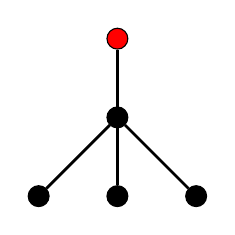
\begin{tikzpicture}
	\begin{pgfonlayer}{nodelayer}
		\node [style=logical_qubit] (0) at (0, -0) {};
		\node [style=auxiliary_qubit] (1) at (0, 1) {};
		\node [style=logical_qubit] (2) at (-1, -1) {};
		\node [style=logical_qubit] (3) at (1, -1) {};
		\node [style=logical_qubit] (4) at (0, -1) {};
	\end{pgfonlayer}
	\begin{pgfonlayer}{edgelayer}
		\draw [style=simple] (1) to (0);
		\draw [style=simple] (2) to (0);
		\draw [style=simple] (3) to (0);
		\draw [style=simple] (4) to (0);
	\end{pgfonlayer}
\end{tikzpicture}

\caption{logical\_fork3.tikz}
\end{figure}


\begin{figure}
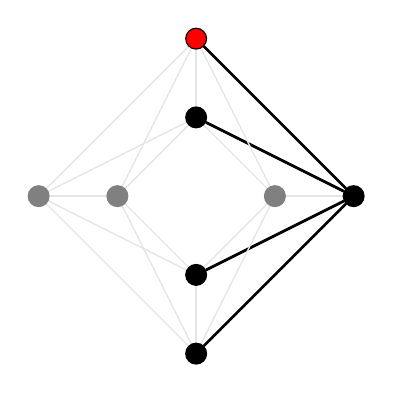
\begin{tikzpicture}
	\begin{pgfonlayer}{nodelayer}
		\node [style=unused_qubit] (0) at (-2, -0) {};
		\node [style=unused_qubit] (1) at (-1, -0) {};
		\node [style=logical_qubit] (2) at (2, -0) {};
		\node [style=auxiliary_qubit] (3) at (0, 2) {};
		\node [style=logical_qubit] (4) at (0, 1) {};
		\node [style=logical_qubit] (5) at (0, -1) {};
		\node [style=logical_qubit] (6) at (0, -2) {};
		\node [style=unused_qubit] (7) at (1, -0) {};
	\end{pgfonlayer}
	\begin{pgfonlayer}{edgelayer}
		\draw [style=simple] (3) to (2);
		\draw [style=unused] (1) to (4);
		\draw [style=unused] (0) to (4);
		\draw [style=simple] (4) to (2);
		\draw [style={unused_added}] (0) to (1);
		\draw [style=unused] (1) to (5);
		\draw [style=simple] (5) to (2);
		\draw [style=unused] (5) to (0);
		\draw [style=unused] (0) to (6);
		\draw [style=simple] (6) to (2);
		\draw [style=unused] (6) to (1);
		\draw [style={unused_added}] (3) to (4);
		\draw [style={unused_added}] (5) to (6);
		\draw [style=unused] (0) to (3);
		\draw [style=unused] (1) to (3);
		\draw [style=unused] (7) to (4);
		\draw [style=unused] (7) to (5);
		\draw [style=unused] (7) to (6);
		\draw [style=unused] (7) to (3);
		\draw [style={unused_added}] (7) to (2);
	\end{pgfonlayer}
\end{tikzpicture}

\caption{logical\_fork3\_inPegasus.tikz}
\end{figure}

Gadgets with adjacency graph corresponding to logical\_fork3.tikz(\scalebox{.25}{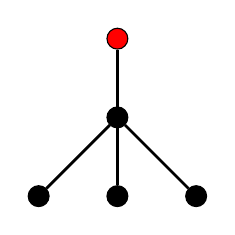
\begin{tikzpicture}
	\begin{pgfonlayer}{nodelayer}
		\node [style=logical_qubit] (0) at (0, -0) {};
		\node [style=auxiliary_qubit] (1) at (0, 1) {};
		\node [style=logical_qubit] (2) at (-1, -1) {};
		\node [style=logical_qubit] (3) at (1, -1) {};
		\node [style=logical_qubit] (4) at (0, -1) {};
	\end{pgfonlayer}
	\begin{pgfonlayer}{edgelayer}
		\draw [style=simple] (1) to (0);
		\draw [style=simple] (2) to (0);
		\draw [style=simple] (3) to (0);
		\draw [style=simple] (4) to (0);
	\end{pgfonlayer}
\end{tikzpicture}
}):

\begin{itemize}
\item NTR-ABCB
\end{itemize}

\begin{figure}
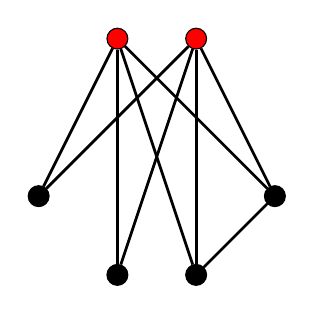
\begin{tikzpicture}
	\begin{pgfonlayer}{nodelayer}
		\node [style=logical_qubit] (0) at (-1, -0) {};
		\node [style=logical_qubit] (1) at (0, -1) {};
		\node [style=logical_qubit] (2) at (2, -0) {};
		\node [style=auxiliary_qubit] (3) at (0, 2) {};
		\node [style=auxiliary_qubit] (4) at (1, 2) {};
		\node [style=logical_qubit] (5) at (1, -1) {};
	\end{pgfonlayer}
	\begin{pgfonlayer}{edgelayer}
		\draw [style=simple] (3) to (2);
		\draw [style=simple] (1) to (4);
		\draw [style=simple] (0) to (4);
		\draw [style=simple] (4) to (2);
		\draw [style=simple] (0) to (3);
		\draw [style=simple] (1) to (3);
		\draw [style=simple] (5) to (4);
		\draw [style=simple] (5) to (3);
		\draw [style=simple] (5) to (2);
	\end{pgfonlayer}
\end{tikzpicture}

\caption{2aux\_to\_all4\_1conn.tikz}
\end{figure}

\begin{figure}
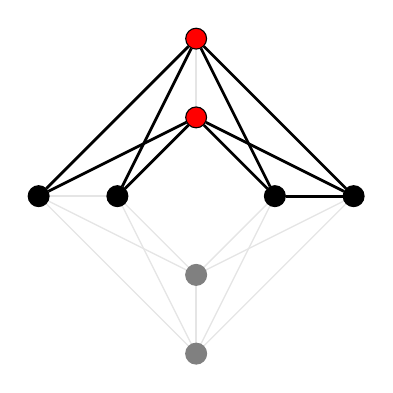
\begin{tikzpicture}
	\begin{pgfonlayer}{nodelayer}
		\node [style=logical_qubit] (0) at (-2, -0) {};
		\node [style=logical_qubit] (1) at (-1, -0) {};
		\node [style=logical_qubit] (2) at (2, -0) {};
		\node [style=auxiliary_qubit] (3) at (0, 2) {};
		\node [style=auxiliary_qubit] (4) at (0, 1) {};
		\node [style=unused_qubit] (5) at (0, -1) {};
		\node [style=unused_qubit] (6) at (0, -2) {};
		\node [style=logical_qubit] (7) at (1, -0) {};
	\end{pgfonlayer}
	\begin{pgfonlayer}{edgelayer}
		\draw [style=simple] (3) to (2);
		\draw [style=simple] (1) to (4);
		\draw [style=simple] (0) to (4);
		\draw [style=simple] (4) to (2);
		\draw [style={unused_added}] (0) to (1);
		\draw [style=unused] (1) to (5);
		\draw [style=unused] (5) to (2);
		\draw [style=unused] (5) to (0);
		\draw [style=unused] (0) to (6);
		\draw [style=unused] (6) to (2);
		\draw [style=unused] (6) to (1);
		\draw [style={unused_added}] (3) to (4);
		\draw [style={unused_added}] (5) to (6);
		\draw [style=simple] (0) to (3);
		\draw [style=simple] (1) to (3);
		\draw [style=simple] (7) to (4);
		\draw [style=unused] (7) to (5);
		\draw [style=unused] (7) to (6);
		\draw [style=simple] (7) to (3);
		\draw [style=added] (7) to (2);
	\end{pgfonlayer}
\end{tikzpicture}

\caption{2aux\_to\_all4\_1conn\_inPegasus.tikz}
\end{figure}

\begin{figure}
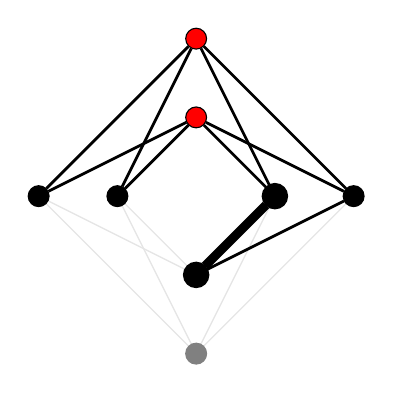
\begin{tikzpicture}
	\begin{pgfonlayer}{nodelayer}
		\node [style=logical_qubit] (0) at (-2, -0) {};
		\node [style=logical_qubit] (1) at (-1, -0) {};
		\node [style=logical_qubit] (2) at (2, -0) {};
		\node [style=auxiliary_qubit] (3) at (0, 2) {};
		\node [style=auxiliary_qubit] (4) at (0, 1) {};
		\node [style=emb_logical_qubit] (5) at (0, -1) {};
		\node [style=unused_qubit] (6) at (0, -2) {};
		\node [style=emb_logical_qubit] (7) at (1, -0) {};
	\end{pgfonlayer}
	\begin{pgfonlayer}{edgelayer}
		\draw [style=unused] (0) to (6);
		\draw [style=unused] (6) to (2);
		\draw [style=unused] (6) to (1);
		\draw [style=unused] (1) to (5);
		\draw [style=unused] (7) to (6);
		\draw [style=unused] (5) to (0);
		\draw [style=simple] (3) to (2);
		\draw [style=simple] (1) to (4);
		\draw [style=simple] (0) to (4);
		\draw [style=simple] (4) to (2);
		
		\draw [style=simple] (5) to (2);
		
		
		\draw [style=simple] (0) to (3);
		\draw [style=simple] (1) to (3);
		\draw [style=simple] (7) to (4);
		\draw [style={embedding}] (7) to (5);
		
		\draw [style=simple] (7) to (3);
	\end{pgfonlayer}
\end{tikzpicture}

\caption{2aux\_to\_all4\_1conn\_inChimera.tikz}
\end{figure}

Gadgets with adjacency graph corresponding to 2aux\_to\_all4\_1conn.tikz(\scalebox{.25}{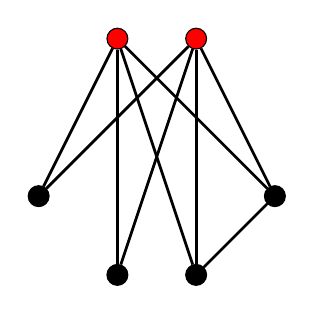
\begin{tikzpicture}
	\begin{pgfonlayer}{nodelayer}
		\node [style=logical_qubit] (0) at (-1, -0) {};
		\node [style=logical_qubit] (1) at (0, -1) {};
		\node [style=logical_qubit] (2) at (2, -0) {};
		\node [style=auxiliary_qubit] (3) at (0, 2) {};
		\node [style=auxiliary_qubit] (4) at (1, 2) {};
		\node [style=logical_qubit] (5) at (1, -1) {};
	\end{pgfonlayer}
	\begin{pgfonlayer}{edgelayer}
		\draw [style=simple] (3) to (2);
		\draw [style=simple] (1) to (4);
		\draw [style=simple] (0) to (4);
		\draw [style=simple] (4) to (2);
		\draw [style=simple] (0) to (3);
		\draw [style=simple] (1) to (3);
		\draw [style=simple] (5) to (4);
		\draw [style=simple] (5) to (3);
		\draw [style=simple] (5) to (2);
	\end{pgfonlayer}
\end{tikzpicture}
}):

\begin{itemize}
\item positive term reduction
\end{itemize}

\begin{figure}
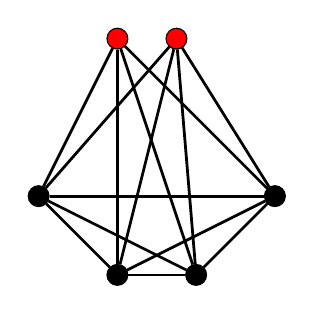
\begin{tikzpicture}
	\begin{pgfonlayer}{nodelayer}
		\node [style=logical_qubit] (0) at (-1, -0) {};
		\node [style=logical_qubit] (1) at (2, -0) {};
		\node [style=auxiliary_qubit] (2) at (0, 2) {};
		\node [style=auxiliary_qubit] (3) at (0.75, 2) {};
		\node [style=logical_qubit] (4) at (0, -1) {};
		\node [style=logical_qubit] (5) at (1, -1) {};
	\end{pgfonlayer}
	\begin{pgfonlayer}{edgelayer}
		\draw [style=simple] (2) to (1);
		\draw [style=simple] (0) to (3);
		\draw [style=simple] (3) to (1);
		\draw [style=simple] (4) to (1);
		\draw [style=simple] (0) to (2);
		\draw [style=simple] (5) to (3);
		\draw [style=simple] (5) to (4);
		\draw [style=simple] (5) to (2);
		\draw [style=simple] (5) to (1);
		\draw [style=simple] (4) to (3);
		\draw [style=simple] (4) to (2);
		\draw [style=simple] (4) to (0);
		\draw [style=simple] (0) to (5);
		\draw [style=simple] (0) to (1);
	\end{pgfonlayer}
\end{tikzpicture}

\caption{2aux\_to\_all4\_allConn.tikz}
\end{figure}

\begin{figure}
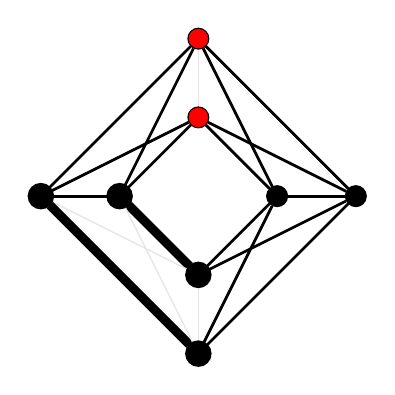
\begin{tikzpicture}
	\begin{pgfonlayer}{nodelayer}
		\node [style=emb_logical_qubit] (0) at (-2, -0) {};
		\node [style=emb_logical_qubit] (1) at (-1, -0) {};
		\node [style=logical_qubit] (2) at (2, -0) {};
		\node [style=auxiliary_qubit] (3) at (0, 2) {};
		\node [style=auxiliary_qubit] (4) at (0, 1) {};
		\node [style=emb_logical_qubit] (5) at (0, -1) {};
		\node [style=emb_logical_qubit] (6) at (0, -2) {};
		\node [style=logical_qubit] (7) at (1, -0) {};
	\end{pgfonlayer}
	\begin{pgfonlayer}{edgelayer}
		\draw [style=simple] (3) to (2);
		\draw [style=simple] (1) to (4);
		\draw [style=simple] (0) to (4);
		\draw [style=simple] (4) to (2);
		\draw [style=added] (0) to (1);
		\draw [style={embedding}] (1) to (5);
		\draw [style=simple] (5) to (2);
		\draw [style=unused] (5) to (0);
		\draw [style={embedding}] (0) to (6);
		\draw [style=simple] (6) to (2);
		\draw [style=unused] (6) to (1);
		\draw [style={unused_added}] (3) to (4);
		\draw [style={unused_added}] (5) to (6);
		\draw [style=simple] (0) to (3);
		\draw [style=simple] (1) to (3);
		\draw [style=simple] (7) to (4);
		\draw [style=simple] (7) to (5);
		\draw [style=simple] (7) to (6);
		\draw [style=simple] (7) to (3);
		\draw [style=added] (7) to (2);
	\end{pgfonlayer}
\end{tikzpicture}

\caption{2aux\_to\_all4\_allConn\_inPegasus.tikz}
\end{figure}



Gadgets with adjacency graph corresponding to 2aux\_to\_all4\_allConn.tikz(\scalebox{.25}{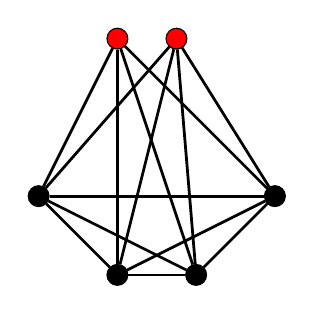
\begin{tikzpicture}
	\begin{pgfonlayer}{nodelayer}
		\node [style=logical_qubit] (0) at (-1, -0) {};
		\node [style=logical_qubit] (1) at (2, -0) {};
		\node [style=auxiliary_qubit] (2) at (0, 2) {};
		\node [style=auxiliary_qubit] (3) at (0.75, 2) {};
		\node [style=logical_qubit] (4) at (0, -1) {};
		\node [style=logical_qubit] (5) at (1, -1) {};
	\end{pgfonlayer}
	\begin{pgfonlayer}{edgelayer}
		\draw [style=simple] (2) to (1);
		\draw [style=simple] (0) to (3);
		\draw [style=simple] (3) to (1);
		\draw [style=simple] (4) to (1);
		\draw [style=simple] (0) to (2);
		\draw [style=simple] (5) to (3);
		\draw [style=simple] (5) to (4);
		\draw [style=simple] (5) to (2);
		\draw [style=simple] (5) to (1);
		\draw [style=simple] (4) to (3);
		\draw [style=simple] (4) to (2);
		\draw [style=simple] (4) to (0);
		\draw [style=simple] (0) to (5);
		\draw [style=simple] (0) to (1);
	\end{pgfonlayer}
\end{tikzpicture}
}):

\begin{itemize}
\item PTR-Ishikawa
\end{itemize}

\begin{figure}
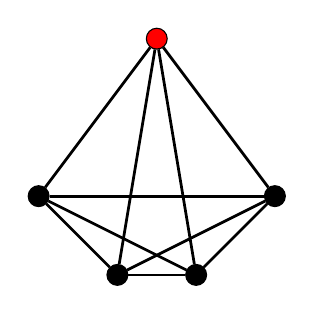
\begin{tikzpicture}
	\begin{pgfonlayer}{nodelayer}
		\node [style=logical_qubit] (0) at (2, -0) {};
		\node [style=auxiliary_qubit] (1) at (0.5, 2) {};
		\node [style=logical_qubit] (2) at (0, -1) {};
		\node [style=logical_qubit] (3) at (-1, -0) {};
		\node [style=logical_qubit] (4) at (1, -1) {};
	\end{pgfonlayer}
	\begin{pgfonlayer}{edgelayer}
		\draw [style=simple] (1) to (0);
		\draw [style=simple] (2) to (0);
		\draw [style=simple] (3) to (0);
		\draw [style=simple] (4) to (2);
		\draw [style=simple] (4) to (3);
		\draw [style=simple] (4) to (1);
		\draw [style=simple] (4) to (0);
		\draw [style=simple] (2) to (3);
		\draw [style=simple] (3) to (1);
		\draw [style=simple] (2) to (1);
	\end{pgfonlayer}
\end{tikzpicture}

\caption{aux\_to\_all4\_allConn.tikz}
\end{figure}

\begin{figure}
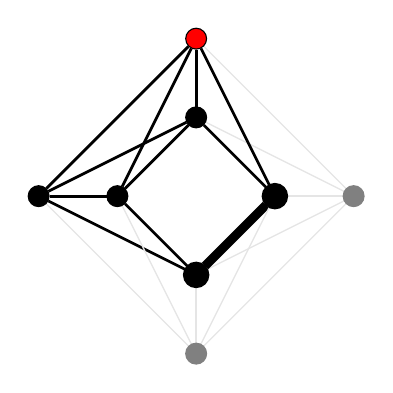
\begin{tikzpicture}
	\begin{pgfonlayer}{nodelayer}
		\node [style=logical_qubit] (0) at (-2, -0) {};
		\node [style=logical_qubit] (1) at (-1, -0) {};
		\node [style=unused_qubit] (2) at (2, -0) {};
		\node [style=auxiliary_qubit] (3) at (0, 2) {};
		\node [style=logical_qubit] (4) at (0, 1) {};
		\node [style={emb_logical_qubit}] (5) at (0, -1) {};
		\node [style=unused_qubit] (6) at (0, -2) {};
		\node [style={emb_logical_qubit}] (7) at (1, -0) {};
	\end{pgfonlayer}
	\begin{pgfonlayer}{edgelayer}
		\draw [style=unused] (3) to (2);
		\draw [style=simple] (1) to (4);
		\draw [style=simple] (0) to (4);
		\draw [style=unused] (4) to (2);
		\draw [style=added] (0) to (1);
		\draw [style=simple] (1) to (5);
		\draw [style=unused] (5) to (2);
		\draw [style=simple] (5) to (0);
		\draw [style=unused] (0) to (6);
		\draw [style=unused] (6) to (2);
		\draw [style=unused] (6) to (1);
		\draw [style=added] (3) to (4);
		\draw [style={unused_added}] (5) to (6);
		\draw [style=simple] (0) to (3);
		\draw [style=simple] (1) to (3);
		\draw [style=simple] (7) to (4);
		\draw [style={embedding}] (7) to (5);
		\draw [style=unused] (7) to (6);
		\draw [style=simple] (7) to (3);
		\draw [style={unused_added}] (7) to (2);
	\end{pgfonlayer}
\end{tikzpicture}

\caption{aux\_to\_all4\_allConn\_inPegasus.tikz}
\end{figure}

\begin{figure}
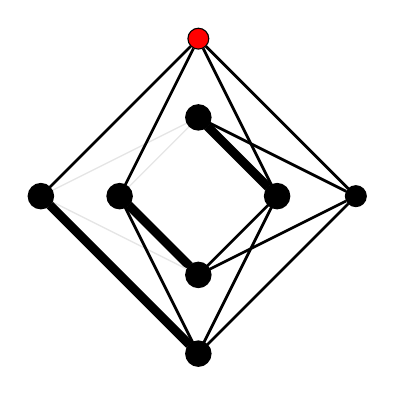
\begin{tikzpicture}
	\begin{pgfonlayer}{nodelayer}
		\node [style=emb_logical_qubit] (0) at (-2, -0) {};
		\node [style=emb_logical_qubit] (1) at (-1, -0) {};
		\node [style=logical_qubit] (2) at (2, -0) {};
		\node [style=auxiliary_qubit] (3) at (0, 2) {};
		\node [style=emb_logical_qubit] (4) at (0, 1) {};
		\node [style=emb_logical_qubit] (5) at (0, -1) {};
		\node [style=emb_logical_qubit] (6) at (0, -2) {};
		\node [style=emb_logical_qubit] (7) at (1, -0) {};
	\end{pgfonlayer}
	\begin{pgfonlayer}{edgelayer}
		\draw [style=simple] (3) to (2);
		\draw [style=unused] (1) to (4);
		\draw [style=unused] (0) to (4);
		\draw [style=simple] (4) to (2);
		\draw [style={embedding}] (1) to (5);
		\draw [style=simple] (5) to (2);
		\draw [style=unused] (5) to (0);
		\draw [style={embedding}] (0) to (6);
		\draw [style=simple] (6) to (2);
		\draw [style=simple] (6) to (1);
		\draw [style=simple] (0) to (3);
		\draw [style=simple] (1) to (3);
		\draw [style={embedding}] (7) to (4);
		\draw [style=simple] (7) to (5);
		\draw [style=simple] (7) to (6);
		\draw [style=simple] (7) to (3);
	\end{pgfonlayer}
\end{tikzpicture}

\caption{aux\_to\_all4\_allConn\_inChimera.tikz}
\end{figure}

Gadgets with adjacency graph corresponding to aux\_to\_all4\_allConn.tikz(\scalebox{.25}{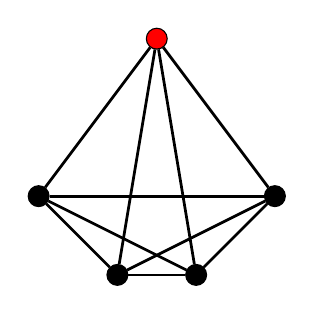
\begin{tikzpicture}
	\begin{pgfonlayer}{nodelayer}
		\node [style=logical_qubit] (0) at (2, -0) {};
		\node [style=auxiliary_qubit] (1) at (0.5, 2) {};
		\node [style=logical_qubit] (2) at (0, -1) {};
		\node [style=logical_qubit] (3) at (-1, -0) {};
		\node [style=logical_qubit] (4) at (1, -1) {};
	\end{pgfonlayer}
	\begin{pgfonlayer}{edgelayer}
		\draw [style=simple] (1) to (0);
		\draw [style=simple] (2) to (0);
		\draw [style=simple] (3) to (0);
		\draw [style=simple] (4) to (2);
		\draw [style=simple] (4) to (3);
		\draw [style=simple] (4) to (1);
		\draw [style=simple] (4) to (0);
		\draw [style=simple] (2) to (3);
		\draw [style=simple] (3) to (1);
		\draw [style=simple] (2) to (1);
	\end{pgfonlayer}
\end{tikzpicture}
}):

\begin{itemize}
\item PTR-BCR-2
\item PTR-BCR-4
\end{itemize}

\begin{figure}
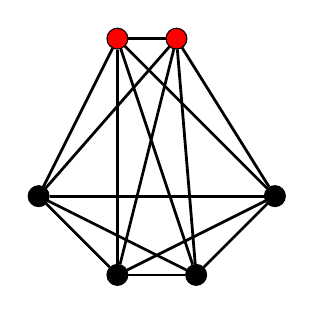
\begin{tikzpicture}
	\begin{pgfonlayer}{nodelayer}
		\node [style=logical_qubit] (0) at (-1, -0) {};
		\node [style=logical_qubit] (1) at (2, -0) {};
		\node [style=auxiliary_qubit] (2) at (0, 2) {};
		\node [style=auxiliary_qubit] (3) at (0.75, 2) {};
		\node [style=logical_qubit] (4) at (0, -1) {};
		\node [style=logical_qubit] (5) at (1, -1) {};
	\end{pgfonlayer}
	\begin{pgfonlayer}{edgelayer}
		\draw [style=simple] (2) to (1);
		\draw [style=simple] (0) to (3);
		\draw [style=simple] (3) to (1);
		\draw [style=simple] (4) to (1);
		\draw [style=simple] (0) to (2);
		\draw [style=simple] (5) to (3);
		\draw [style=simple] (5) to (4);
		\draw [style=simple] (5) to (2);
		\draw [style=simple] (5) to (1);
		\draw [style=simple] (2) to (3);
		\draw [style=simple] (4) to (3);
		\draw [style=simple] (4) to (2);
		\draw [style=simple] (4) to (0);
		\draw [style=simple] (0) to (5);
		\draw [style=simple] (0) to (1);
	\end{pgfonlayer}
\end{tikzpicture}

\caption{2auxConn\_to\_all4\_allConn.tikz}
\end{figure}

\begin{figure}
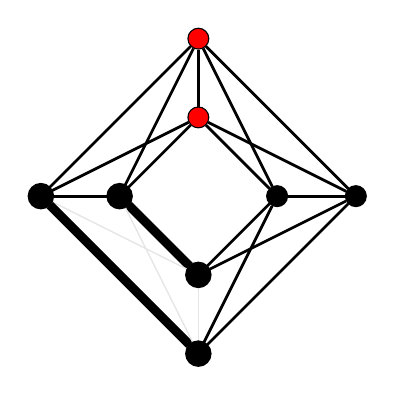
\begin{tikzpicture}
	\begin{pgfonlayer}{nodelayer}
		\node [style=emb_logical_qubit] (0) at (-2, -0) {};
		\node [style=emb_logical_qubit] (1) at (-1, -0) {};
		\node [style=logical_qubit] (2) at (2, -0) {};
		\node [style=auxiliary_qubit] (3) at (0, 2) {};
		\node [style=auxiliary_qubit] (4) at (0, 1) {};
		\node [style=emb_logical_qubit] (5) at (0, -1) {};
		\node [style=emb_logical_qubit] (6) at (0, -2) {};
		\node [style=logical_qubit] (7) at (1, -0) {};
	\end{pgfonlayer}
	\begin{pgfonlayer}{edgelayer}
		\draw [style=simple] (3) to (2);
		\draw [style=simple] (1) to (4);
		\draw [style=simple] (0) to (4);
		\draw [style=simple] (4) to (2);
		\draw [style=added] (0) to (1);
		\draw [style={embedding}] (1) to (5);
		\draw [style=simple] (5) to (2);
		\draw [style=unused] (5) to (0);
		\draw [style={embedding}] (0) to (6);
		\draw [style=simple] (6) to (2);
		\draw [style=unused] (6) to (1);
		\draw [style={unused_added}] (5) to (6);
		\draw [style=simple] (0) to (3);
		\draw [style=simple] (1) to (3);
		\draw [style=simple] (7) to (4);
		\draw [style=simple] (7) to (5);
		\draw [style=simple] (7) to (6);
		\draw [style=simple] (7) to (3);
		\draw [style=added] (7) to (2);
		\draw [style=added] (3) to (4);
	\end{pgfonlayer}
\end{tikzpicture}

\caption{2auxConn\_to\_all4\_allConn\_inPegasus.tikz}
\end{figure}

Gadgets with adjacency graph corresponding to 2auxConn\_to\_all4\_allConn.tikz(\scalebox{.25}{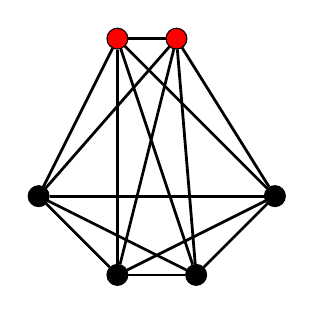
\begin{tikzpicture}
	\begin{pgfonlayer}{nodelayer}
		\node [style=logical_qubit] (0) at (-1, -0) {};
		\node [style=logical_qubit] (1) at (2, -0) {};
		\node [style=auxiliary_qubit] (2) at (0, 2) {};
		\node [style=auxiliary_qubit] (3) at (0.75, 2) {};
		\node [style=logical_qubit] (4) at (0, -1) {};
		\node [style=logical_qubit] (5) at (1, -1) {};
	\end{pgfonlayer}
	\begin{pgfonlayer}{edgelayer}
		\draw [style=simple] (2) to (1);
		\draw [style=simple] (0) to (3);
		\draw [style=simple] (3) to (1);
		\draw [style=simple] (4) to (1);
		\draw [style=simple] (0) to (2);
		\draw [style=simple] (5) to (3);
		\draw [style=simple] (5) to (4);
		\draw [style=simple] (5) to (2);
		\draw [style=simple] (5) to (1);
		\draw [style=simple] (2) to (3);
		\draw [style=simple] (4) to (3);
		\draw [style=simple] (4) to (2);
		\draw [style=simple] (4) to (0);
		\draw [style=simple] (0) to (5);
		\draw [style=simple] (0) to (1);
	\end{pgfonlayer}
\end{tikzpicture}
}):

\begin{itemize}
\item PTR-BCR-3
\end{itemize}

\begin{figure}
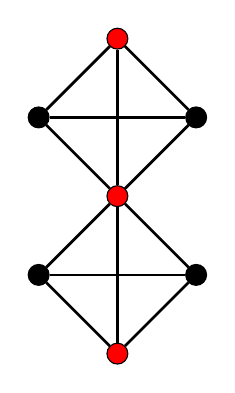
\begin{tikzpicture}
	\begin{pgfonlayer}{nodelayer}
		\node [style=logical_qubit] (0) at (-1, -0) {};
		\node [style=auxiliary_qubit] (1) at (0, 3) {};
		\node [style=logical_qubit] (2) at (-1, 2) {};
		\node [style=auxiliary_qubit] (3) at (0, 1) {};
		\node [style=logical_qubit] (4) at (1, -0) {};
		\node [style=auxiliary_qubit] (5) at (0, -1) {};
		\node [style=logical_qubit] (6) at (1, 2) {};
	\end{pgfonlayer}
	\begin{pgfonlayer}{edgelayer}
		\draw [style=simple] (2) to (1);
		\draw [style=simple] (3) to (1);
		\draw [style=simple] (4) to (0);
		\draw [style=simple] (0) to (5);
		\draw [style=simple] (4) to (5);
		\draw [style=simple] (6) to (3);
		\draw [style=simple] (6) to (2);
		\draw [style=simple] (6) to (1);
		\draw [style=simple] (2) to (3);
		\draw [style=simple] (0) to (3);
		\draw [style=simple] (4) to (3);
		\draw [style=simple] (5) to (3);
	\end{pgfonlayer}
\end{tikzpicture}

\caption{2k4\_shared\_aux.tikz}
\end{figure}

\begin{figure}
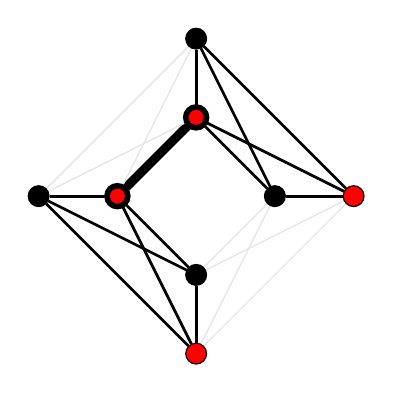
\begin{tikzpicture}
	\begin{pgfonlayer}{nodelayer}
		\node [style=logical_qubit] (0) at (-2, -0) {};
		\node [style=emb_auxiliary_qubit] (1) at (-1, -0) {};
		\node [style=auxiliary_qubit] (2) at (2, -0) {};
		\node [style=logical_qubit] (3) at (0, 2) {};
		\node [style=emb_auxiliary_qubit] (4) at (0, 1) {};
		\node [style=logical_qubit] (5) at (0, -1) {};
		\node [style=auxiliary_qubit] (6) at (0, -2) {};
		\node [style=logical_qubit] (7) at (1, -0) {};
	\end{pgfonlayer}
	\begin{pgfonlayer}{edgelayer}
		\draw [style=simple] (3) to (2);
		\draw [style={embedding}] (1) to (4);
		\draw [style=unused] (0) to (4);
		\draw [style=simple] (4) to (2);
		\draw [style=added] (0) to (1);
		\draw [style=simple] (1) to (5);
		\draw [style=unused] (5) to (2);
		\draw [style=simple] (5) to (0);
		\draw [style=simple] (0) to (6);
		\draw [style=unused] (6) to (2);
		\draw [style=simple] (6) to (1);
		\draw [style=added] (5) to (6);
		\draw [style=unused] (0) to (3);
		\draw [style=unused] (1) to (3);
		\draw [style=simple] (7) to (4);
		\draw [style=unused] (7) to (5);
		\draw [style=unused] (7) to (6);
		\draw [style=simple] (7) to (3);
		\draw [style=added] (7) to (2);
		\draw [style=added] (3) to (4);
	\end{pgfonlayer}
\end{tikzpicture}

\caption{2k4\_shared\_aux\_inPegasus.tikz}
\end{figure}

Gadgets with adjacency graph corresponding to 2k4\_shared\_aux.tikz(\scalebox{.25}{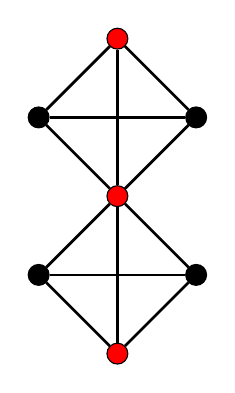
\begin{tikzpicture}
	\begin{pgfonlayer}{nodelayer}
		\node [style=logical_qubit] (0) at (-1, -0) {};
		\node [style=auxiliary_qubit] (1) at (0, 3) {};
		\node [style=logical_qubit] (2) at (-1, 2) {};
		\node [style=auxiliary_qubit] (3) at (0, 1) {};
		\node [style=logical_qubit] (4) at (1, -0) {};
		\node [style=auxiliary_qubit] (5) at (0, -1) {};
		\node [style=logical_qubit] (6) at (1, 2) {};
	\end{pgfonlayer}
	\begin{pgfonlayer}{edgelayer}
		\draw [style=simple] (2) to (1);
		\draw [style=simple] (3) to (1);
		\draw [style=simple] (4) to (0);
		\draw [style=simple] (0) to (5);
		\draw [style=simple] (4) to (5);
		\draw [style=simple] (6) to (3);
		\draw [style=simple] (6) to (2);
		\draw [style=simple] (6) to (1);
		\draw [style=simple] (2) to (3);
		\draw [style=simple] (0) to (3);
		\draw [style=simple] (4) to (3);
		\draw [style=simple] (5) to (3);
	\end{pgfonlayer}
\end{tikzpicture}
}):

\begin{itemize}
\item Two copies of PTR-KZ sharing an auxilla
\item Two copies of z-version of PTR-KZ sharing an auxilla
\end{itemize}






\end{document}
